\newcommand{\urlmathematicatechintro}{https://content.byui.edu/file/664390b8-e9cc-43a4-9f3c-70362f8b9735/1/_zips/316-Tech-Introduction.zip}

After completing this chapter, you should be able to:

\begin{enumerate}
\item Explain how to compute Laplace transforms and inverse Laplace transforms. Use Laplace transforms to solve IVPs.

\item Use and prove both both the $s$-shifting and $t$-shifting theorems. 
\item Express discontinuous functions with the Heaviside function, and use the Heaviside to set up and solve ODEs.
\item Express impulses in terms of the Dirac delta distribution, and use it to set up and solve solve ODEs.
\item Compute convolutions, and show how to use the convolution theorem as an inverse product rule for Laplace transforms.
\end{enumerate}

\marginpar{You may want to download this \href{\urlmathematicatechintro}{Mathematica Technology Introduction} to check your work throughout the entire chapter.}%
You can find additional practice problems in Schaum's Outlines \textit{Differential Equations} by Richard Bronson.
You'll find relevant problems in chapters 21 -24, as well as some extra practice problems at the end of this chapter. 
Do enough of each type that you feel comfortable with the ideas. 

\begin{table}[h]
\begin{center}
\begin{tabular}{cc}
\begin{tabular}[t]{|c|cc|}
\hline
$f(t)$ & $F(s)$ & provided\\
\hline\hline
$1$					&$\dfrac{1}{s}$ 							&$s>0$\\\hline
$t^n$				&$\dfrac{n!}{s^{n+1}}$ 			&$s>0$\\\hline
$e^{at}$		&$\dfrac{1}{s-a}$ 			&$s>a$\\\hline
$y'$					&$sY-y(0)$ 						&\\\hline
$y''$					&$s^2Y-sy(0)-y'(0)$ 						&\\\hline
%$y'''$					&$s^3Y-s^2y(0)-sy'(0)-y''(0)$ 						&\\\hline
$e^{at}f(t)$  &$F(s-a)$ 						&\\\hline
$f(t)*g(t)$  &$F(s)G(s)$ 						&\\\hline
\end{tabular}
&
\begin{tabular}[t]{|c|cc|}
\hline
$f(t)$ & $F(s)$ & provided\\
\hline\hline
$\cos(wt)$  &$\dfrac{s}{s^2+\omega^2}$ 			&$s>0$\\\hline
$\sin(wt)$  &$\dfrac{\omega}{s^2+\omega^2}$ 			&$s>0$\\\hline
$\cosh(wt)$ &$\dfrac{s}{s^2-\omega^2}$ 			&$s>|\omega|$\\\hline
$\sinh(wt)$ &$\dfrac{\omega}{s^2-\omega^2}$ 			&$s>|\omega|$\\\hline
$u(t-a)$  &$\frac{1}{s}e^{-as}$ 						&\\\hline
$\delta(t-a)$  &$e^{-as}$ 						&\\\hline
$f(t-a)u(t-a)$  &$\mathscr{L}(f(t))e^{-as}$ 						&\\
$f(t)u(t-a)$  &$\mathscr{L}(f(t+a))e^{-as}$ 						&\\
\hline
\end{tabular}
\end{tabular}
\end{center}
\caption{Table of Laplace Transforms\label{big laplace table}. Note that the $s$ shifting theorem $\mathscr{L}(e^{at}f(t))=F(s-a)$ has a positive $a$ in the exponent, while the $t$ shifting theorem $\mathscr{L}(f(t-a)u(t-a))=\mathscr{L}(f(t))e^{-as}$ has a negative $a$ in the exponent.
}
\end{table}


You must practice lots of problems to gain a feel for patterns.  Many of the problems in 21-23 are fast. Please take a few minutes every day to just flat out practice with the basics (kind of like when you were learning the times tables - they get really fast if you just practice them). When you feel like you have the basics down, see if you can complete chapters 21 and 22 in less than an hour. If one stumps you, skip it and come back later.  

Once you feel confident, chapters 23 (on convolutions and the heaviside function) and 24 (solving IVPS) will help you use the Laplace transforms to solve ODEs. At the end of this chapter are some additional problems to help you cement your understanding. Table \ref{big laplace table} summarizes the transforms we use most often.




\newcommand{\ReviewSShiftTheorem}{

In this chapter we'll examine how to handle non differentiable changes in an external driving force.  This corresponds to hitting a mass-spring system with a hammer, marching across a bridge, flipping a switch in an electrical network, etc.  We'll find that Laplace transforms provide us with extremely nice tools to solve these types problems.  Before we jump in, let's review how to solve a couple ODEs with Laplace transforms, and perhaps make some connections that we haven't yet made. 

\begin{review*}
 Compute the inverse Laplace transform of $\ds 	\frac{3s+8}{(s+1)^2+16}$. See
\footnote{
We can rewrite $Y$ as 
$$Y 
= \frac{3(s+1)-3+8}{(s+1)^2-16}
= \frac{3(s+1)}{(s+1)^2-16}+\frac{5}{(s+1)^2-16}\frac44.
$$
The inverse Laplace transform is then 
$$y(t) = 3e^{-t}\cosh(4t)+\frac{5}{4}e^{-t}\sinh(4t).$$
}.
\end{review*}







\begin{problem}\label{review of s-shifting theorem}
\marginpar{We've solved inverse transforms such as this one multiple times. If you need to refresh, please head to chapters 21 and 22 in Schaum's, and just practice the problems where answers are provided.}%
 Compute the inverse Laplace transform of $$\ds Y =\frac{5}{(s+3)^3} + \frac{2s+3}{(s+4)^2+9} + \frac{3s+1}{(s+2)^2-49}.$$ 
Use the rules for $\cosh(t)$ and $\sinh(t)$ to tackle the last terms, rather than doing a partial fraction decomposition.  The goal of this problem is to make sure you have the $s$-shifting theorem mastered.
%See 
% \footnote{We have
% $$\begin{array}{rl}
% \ds Y 
% &=\frac{5}{(s+3)^3} + \frac{2(s+4)-8+3}{(s+4)^2+9} + \frac{3(s+2)-6+1}{(s+2)^2-49}\\ 
% &=\frac{5}{(s+3)^3}\frac{2}{2} + \frac{2(s+4)}{(s+4)^2+9} +\frac{-5}{(s+4)^2+9}\frac{3}{3} + \frac{3(s+2)}{(s+2)^2-49}+ \frac{-5}{(s+2)^2-49}\frac{7}{7} 
% \end{array}$$
% The inverse transform is 
% $$\ds y(t) 
% = \frac{5}{2} t^2e^{-3t} 
%  + 2e^{-4t}\cos(3t) 
%  +\frac{-5}{3}e^{-4t}\sin(3t) 
%  +3 e^{-2t}\cosh(7t)
%  +\frac{-5}{7} e^{-2t}\sinh(7t).
% $$
% }.
\end{problem}
}



\newcommand{\CompareDistinctRootsToCoshAndSinh}{
\begin{problem}\label{compare distinct roots with s-shifting and cosh and sinh}
 Consider the IVP $y''+6y'+8y = 0$, $y(0)=2$, $y'(0)=3$.
\begin{enumerate}
 \item Use Laplace transforms to solve the IVP. Use a partial fraction decomposition to write $Y = \frac{A}{s+2}+\frac{B}{S+4}$ and then show that $\ds y(t) = \frac{11}{2}e^{-2t}-\frac{7}{2}e^{-4t}$.  
 \item Instead of using a partial fraction decomposition, instead notice that we could complete the square in the denomoinator to write $s^2+6s+8=(s+3)^2-1$. Use this approach to solve for $y(t)$ and write $y(t)$ as a linear combination of $e^{-3t}\cosh(t)$ and $e^{-3t}\sinh(t)$.
 \item Remember that $\ds \cosh(t) = \frac{e^t+e^{-t}}{2}$ and $\ds \sinh(t) = \frac{e^t-e^{-t}}{2}$. Use this to show how your second solution involving hyperbolic trig functions is really the same as $\ds y(t) = \frac{11}{2}e^{-2t}-\frac{7}{2}e^{-4t}$.
\end{enumerate}
\end{problem}

}

\newcommand{\ExtraCompareDistinctRootsToCoshAndSinh}{
\begin{problem}\label{extra compare distinct roots with s-shifting and cosh and sinh}
 Consider the IVP $y''+7y'+10y = 0$, $y(0)=4$, $y'(0)=-3$.
\begin{enumerate}
 \item Use Laplace transforms and a partial fraction decomposition to solve the IVP. Write your answer as a linear combination of $e^{-2t}$ and $e^{-5t}$.  
 \item Complete the square on $s^2+7s+10$ and use the Laplace transform with $\cosh$ and $\sinh$ rules to solve the IVP.
 \item Which is easier?
\end{enumerate}
\end{problem}

Problems 
\ref{compare distinct roots with s-shifting and cosh and sinh}
and 
\ref{extra compare distinct roots with s-shifting and cosh and sinh}
reviewed the main ideas used in solving ODEs with Laplace transforms.  In addition, these problems illustrate some of the advantages of using the hyperbolic trigonometric functions $\cosh\omega t$ and $\sinh\omega t$. They can greatly simplify computations.

}




\newcommand{\RLCircuitWithBatteryInsertedAndRemovedUsingMovingInitialConditions}{
We can use Laplace transforms to obtain quick solutions to problems with discontinuous external forces. Let's start by examining an $RL$ circuit with a battery, because it keeps the computations simple.

\begin{problem}\label{RLCircuitWithBatteryInsertedAndRemovedUsingMovingInitialConditions}
 Consider an $RL$ circuit with $R=1$ ohms and $L=1$ Henry.  At time zero, there is no battery in the system.  After 2 seconds,  we connect a battery $E=12 V$ to the circuit.  Two seconds after connecting the battery, we disconnect it.  Our goal is to determine the current in the wire exactly 2 second after we disconnect the battery.
\begin{enumerate}
 \item During the first  two seconds, we need to solve the IVP $I'+I=0$ where $I(0)=0$.  Solve this IVP and use your solution to show that the current after 2 seconds is $I(2)=0$.
 \item Between $t=2$ and $t=4$, we know $E=12$.  Solve the IVP $I'+I=12$, $I(2)=0$. Show that $I(4) = 12-12e^{-2}$. This is the current as the battery gets removed.
\WA{http://www.wolframalpha.com/input/?i=y\%27\%2By\%3D12\%2C+y\%282\%29\%3D0}
 \item When we remove the battery, the ODE is $I'+I=0$. We know the initial condition $I(4)=12-12e^{-2}$ from the previous part.  Solve the IVP, and state $I(6)$. 
 \item We can now predict the current at any time $t$. Use piecewise function notation to state the current in the form
$$I(t) = 
\begin{cases}
 0 & 0\leq t< 2\\
 12-12e^{2}e^{-t} & 2\leq t< 4\\
 ? & 4\leq t\\
\end{cases}
.$$ 
\end{enumerate}
\end{problem}

}


\newcommand{\RLCircuitWithBatteryInsertedAndRemovedUsingShifting}{
In Problem \ref{RLCircuitWithBatteryInsertedAndRemovedUsingMovingInitialConditions}, we found the current using the initial conditions $I(0)=0$, $I(2)=0$, and $I(4)=?$. Another way to tackle this problem is to move our reference frame, letting $t=0$ correspond to the beginning of each change. The computations are often simpler, and we then just have to shift the reference frame back when we finish the problem. 

\begin{problem}\label{RLCircuitWithBatteryInsertedAndRemovedUsingShifting}
 Consider again the same $RL$ circuit with $R=1$ ohms and $L=1$ Henry.  At time zero, there is no battery in the system.  After 2 seconds,  we connect a battery $E=12 V$ to the circuit.  Two seconds after connecting the battery, we disconnect it.  Our goal is to determine the current in the wire exactly 2 second after we disconnect the battery. We'll solve this problem by always making $t=0$ the start of each IVP.
\begin{enumerate}
 \item During the first  two seconds, we need to solve the IVP $I'+I=0$ where $I(0)=0$.  Solve this IVP and use your solution to show that the current after 2 seconds is $I(2)=0$.
 \item Between 2 and 4 seconds, we know $E=12$. Letting $t=0$ correspond to 2 seconds, solve the IVP $I'+I=12$, $I(0)=0$. What is $I(2)$, the current right when the battery gets removed?
 \item When we remove the battery, the ODE is $I'+I=0$. Let $t=0$ correspond to 4 seconds, and then we know the initial condition $I(0)$ from the last part.  Solve the IVP, and state the current $I(2)$ after 6 seconds. 
 \item Use piecewise function notation to state the current at any time $t$. Remember to shift your solutions from the 2nd and 3rd part. Your answer will look like 
$$I(t) = 
\begin{cases}
 0 & 0\leq t< 2\\
 12-12e^{-(t-2)} & 2\leq t< 4\\
 ? & 4\leq t\\
\end{cases}
.$$ 
\end{enumerate}
\end{problem}

}








\newcommand{\IntroductionToGraphingPiecewiseDefineFunctions}{
The electromotive force $E(t)$ in Problem \ref{RLCircuitWithBatteryInsertedAndRemovedUsingMovingInitialConditions} was a piecewise defined force. It was zero, then 12, then 0. Using piecewise notation, we would write this as
$$E(t) =
\begin{cases}
 0 & 0\leq t<2\\
 12 & 2\leq t<4\\
 0 & 4\leq t
\end{cases}
,$$
and we could graph the function $E(t)$ using the figure to the right.
\marginpar{
\begin{tikzpicture}[scale=.5]
%\draw[step=1cm,gray,very thin,dashed] (-1,-1) grid (7,3);
\draw (-1,0) -- (7,0);
\draw (0,-1) -- (0,3);
\draw[very thick] (0,0) -- (2,0);
\draw[dashed] (2,0) -- (2,2);
\draw[very thick] (2,2) -- (4,2);
\draw[dashed] (4,2) -- (4,0);
\draw[very thick] (4,0) -- (7,0);
\end{tikzpicture}
}
We need a nice clean way to work with piecewise defined external forces.  We also need to become comfortable graphing and working with these kinds of forces.

\begin{problem}
% Give them a piecewise defined function, have them graph it.  Then give them a graph, and have them define the function.
Consider the functions 
$$
f(t) = 
\begin{cases}
 2t & 0\leq t< 2\\
 -t^2+4t & 2\leq t< 4\\
 18-3t& 4\leq t< 6\\
 t^2-12t+35& 6\leq t< 8
\end{cases}
\quad\text{and}
\quad
g(t) = 
\begin{cases}
 2t & 0\leq t< 2\\
 4-(t-2)^2 & 2\leq t< 4\\
 6-3(t-4)& 4\leq t< 6\\
 (t-6)^2-1& 6\leq t< 8
\end{cases}.
$$
\begin{enumerate}
 \item Graph $f(t)$ in the $ty$ plane. 
 \item Graph $g(t)$ in the $ty$ plane. 
 \item Graph $y=2t$, $y=4-t^2$, $y=6-3t$, and $y=t^2-1$ in the $ty$ plane.  What does this have to do with the above?
\end{enumerate}

\end{problem}

}



%\subsection{The Heaviside function $u(t-a)$}

\newcommand{\DefinitionOfHeavisideAndGraphOfAFewFunctions}{
We now define the key function that allows us to work with piecewise defined functions.  Some people call this the Heaviside function, some call it the unit step function. This is a simple function that jumps up a single unit at a specified value of $t$. 
\begin{definition}[Heaviside or Unit Step Function]
\marginpar{In our work, it won't matter what we define $u(0)$ to equal. Here, we define $u(0)=1$, but we could have just as easily define $u(0)=0$ or $u(0)=1/2$.  This last option, the 1/2, comes in handy when working with Fourier series.}
We define the Heaviside, or unit step function, to be the function
$$u(t) = \begin{cases}0 &t<0 \\ 1 &t\geq 0\end{cases}.$$ 
We'll most often shift this function right $a$ units, so we replace $t$ with $t-a$, which means we could write
$$u(t-a) = \begin{cases}0 &t-a<0 \\ 1 &t-a\geq 0\end{cases}\quad \quad \text{or}\quad u(t-a)= \begin{cases}0 &t<a \\ 1 &t\geq a\end{cases}.$$ 
\end{definition}
Why does this function matter.  It's like an on/off function.  If you multiply $f(t)$ by $u(t-a)$, then the function $f(t)u(t-a)$ is zero to the left of $a$, and is equal to $f(t)$ after $a$. If $a=3$, then look below for the graph of $y=u(t-3)$.
\marginpar{Mathematica uses the name ``HeavisideTheta'' for the Heaviside function.  You'll see the symbol $\theta$ show up as the name of a function. }
\begin{center}
\begin{tikzpicture}[xscale=1,yscale=1]
\draw[very thick,<-,gray] (-1,0)--(3,0);
\draw[very thick,->,gray] (3,1)--(8,1);
\draw[->,gray] (0,0)--(0,2);
\draw[->,gray] (0,0)--(0,-1);
\draw[->,gray] (0,0)--(-1,0);
\draw[->,gray] (0,0)--(9,0);
\foreach \x in {0,...,8}
	\draw[gray] (\x,4pt) -- (\x,-4pt);
\foreach \y in {0,...,1}
	\draw[gray] (2pt,\y) -- (-2pt,\y);
\path (5,1.5) node {$y=u(t-3)$};
\draw (3,0) circle (3pt);
\filldraw (3,1) circle (3pt);
\end{tikzpicture}  
\end{center}
  
\begin{problem}
 Construct a graph of each of the following:
\begin{enumerate}
 \item $f(t) = u(t-4) - u(t-7)$\marginpar{WolframAlpha and I are having issues when it comes to plotting Heavisides.  I can plot the first one just fine, but as soon as I times it by $(10-t)$, it tries to plot a surface.  As such, \href{http://aleph.sagemath.org/?z=eJwrSyzSUC9R1-RK0yjRtNUwNNAt0dTSyEhNLMsszkxJ1SjRNdHUReaaa2pycRXk5JdogHToaJToGOhYaGoCAP0RFH0=&lang=sage}{please use this link to Sage to check your work.} Make sure you can explain how the graphs are made (not just give them).}
 \item $g(t) = (10-t)(u(t-4) - u(t-7))$
 \item $h(t) = (10-(t-4))(u(t-4) - u(t-7))$ (How does this differ from the previous?)
 \item $k(t) = t^2 (u(t-3) - u(t-5))$
 \item $l(t) = (t-3)^2( u(t-3) - u(t-5))$ (How does this differ from the previous?)
\end{enumerate}
\href{http://aleph.sagemath.org/?z=eJwrSyzSUC9R1-RK0yjRtNUwNNAt0dTSyEhNLMsszkxJ1SjRNdHUReaaa2pycRXk5JdogHToaJToGOhYaGoCAP0RFH0=&lang=sage}{Make sure you check your solution by following the link to Sage.}
\end{problem}

}


\newcommand{\GettingFromAGraphToAHeavisideFunction}{
\begin{problem}
% I need something that would show them the reason for $t$ shifting.  Have them concatenate 3 graphs. Give them some crazy ugly thing that is TONS simpler if you first shift each piece.  Then graph it. 
The graphs of $f(t)=9-t^2$ for $0\leq t\leq3$, and $g(t)=3t$ for $0\leq t\leq 2$, and $h(t) = 6-2t$ for $0\leq t\leq 2$ are connected together (when one ends, the others starts) to give the following graph.
\begin{center}
\begin{tikzpicture}[xscale=.5,yscale=.2]
\draw plot[variable=\t,samples=20,domain=0:3] ({\t},{9-\t*\t});
\draw plot[variable=\t,samples=20,domain=3:5] ({\t},{3*(\t-3)});
\draw plot[variable=\t,samples=20,domain=5:8] ({\t},{6-2*(\t-5)});
\draw[->,gray] (0,0)--(0,10);
\draw[->,gray] (0,0)--(0,-1);
\draw[->,gray] (0,0)--(-1,0);
\draw[->,gray] (0,0)--(11,0);
\foreach \x in {-1,...,10}
	\draw[gray] (\x,4pt) -- (\x,-4pt);
\foreach \y in {-1,...,9}
	\draw[gray] (2pt,\y) -- (-2pt,\y);
\end{tikzpicture}  
\end{center}
\begin{enumerate}
 \item Write this function using piecewise function notation.
 \item Write this function using Heaviside notation. You'll want to use the idea that $u(t-a)-u(t-b)$ turns a function on at $a$ and off at $b$. 
 \item When you think you have the function, \href{http://aleph.sagemath.org/?z=eJwrSyzSUC9R1-RK0yjRtNUwNNAt0dTSyEhNLMsszkxJ1SjRNdHUReaaa2pycRXk5JdogHToaJToGOhYaGoCAP0RFH0=&lang=sage}{use this Sage link to check if you are correct} (you'll have to type in your function). 

 Feel free to use Mathematica instead, if you have downloaded and installed it.  Remember that BYU-I students can now install Mathematica on their personal machines for free. Please head to I-Learn for instructions.  You can then download this \href{https://content.byui.edu/file/664390b8-e9cc-43a4-9f3c-70362f8b9735/1/_zips/316-Tech-Introduction.zip}{Mathematica Technology Introduction}, and you'll see how to code HeavisideTheta functions in Mathematica. 
\end{enumerate}
\end{problem}

Did you notice in your work above that it was a lot easier to graph a piecewise defined function when everything was shifted to the starting point.  It's much easier to graph $f(t-a)u(t-a)$ than it is to graph $f(t)u(t-a)$.  We'll find that this remains true as well, when we start applying Laplace transforms.  

}


\newcommand{\DevelopLaplaceTransformOfHeavisideFunction}{
It's time to look at the Laplace transform of the Heaviside function. This problem is the key to why Laplace transforms work so nicely with piecewise defined functions.  We'll compute the Laplace transform of both $f(t-a)u(t-a)$ and $f(t)u(t-a)$.  Then we'll practice on a few problems.

\begin{problem}[$t$-shifting Theorem]
 Suppose that $y=f(t)$ is a function for which you can find the Laplace transform.
\begin{enumerate}
 \item Show, using the definition of the Laplace transform, that we have
$$\mathscr{L}\{f(t-a)u(t-a)\} = \mathscr{L}\{f(t)\}e^{-as}.$$
 In particular, this means that $\mathscr{L}\{1u(t-a)\}=\frac{1}{s}e^{-as}$.  
\item Then show that
$$\mathscr{L}\{f(t)u(t-a)\} = \mathscr{L}\{f(t+a)\}e^{-as}.$$
\end{enumerate}
[Hint: For the first part, just write down the definition of the Laplace transform. You'll have to do a substitution $w=t-a$. Remember that $u(t-a)=0$ if you are below $a$, which should allow you to remove $u(t-a)$ from any integral, after updating the bounds. In particular, you know that $$\int_0^\infty e^{-st}f(t-a)u(t-a)dt=\int_0^a e^{-st}f(t-a)(0)dt+\int_a^\infty e^{-st}f(t-a)(1)dt = 0+\int_a^\infty e^{-st}f(t-a)dt.$$]
 
\end{problem}

}

\newcommand{\PracticeForwardLaplaceOfHeaviside}{
\begin{problem}
 Compute the Laplace transforms of each of the following functions. \marginpar{See Schaum's chapter 24 for lots more practice.  Please do a bunch of these until you feel like you have the idea down.  Each problem takes just a tiny bit of time. Unless you practice this a bunch, you'll be lost and spend gobs of time on the upcoming problems.}
 \begin{enumerate}
  \item $f(t) = 3u(t-4)$
  \item $f(t) = 3(t-4)\,u(t-4)$
  \item $f(t) = 3t\,u(t-4)$ [Hint: $3t=3(t-4)+12$]
  \item $f(t) = (t-3)^2u(t-3)$
  \item $f(t) = t^2(u(t-2)-u(t-5))$
 \end{enumerate}
\end{problem}

}

\newcommand{\PracticeInverseLaplaceOfHeaviside}{
\begin{problem}
 Compute the inverse Laplace transform of each of the following functions.
 \begin{enumerate}
\begin{multicols}{4}  \item $\dfrac{4}{s^3}e^{-2s}$
  \item $\dfrac{4}{(s+5)^3}e^{-2s}$
  \item $\dfrac{2s+1}{s^2+9}e^{-\pi s/6}$
  \item $\dfrac{3s+4}{(s+2)^2+16}e^{-5s}$
 \end{multicols}
 \end{enumerate}
\end{problem}

}


\newcommand{\FirstSimpleRLCircuitIVP}{
We are now ready to solve Laplace transform problems with the Heaviside function.  The simplest example is an $RL$ circuit.
\begin{problem}
 Consider an $RL$ circuit with $R=4$ and $L=1$. At $t=0$ there is no current in the wire.  Two seconds later ($t=2$), we connect a 9V battery to the circuit.  Three seconds later ($t=5$) we remove the battery.  This gives us the electromotive force as $E(t) = 9(u(t-2)-u(t-5))$.  
 We need to solve the IVP
 $$1I'+4I=9(u(t-2)-u(t-5)), \quad I(0)=0.$$
 Use Laplace transforms to predict the current $I(t)$ at any time $t$. Check your answer with technology. 
 [Hint: You'll want to ignore the $e^{-as}$ terms when you perform any needed partial fraction decompositions.]
\end{problem}

}


\newcommand{\RLCircuitWithRampUpForce}{
\begin{problem}
\marginpar{Remember that the key ODE is $LI'+RI+\frac{1}{C}Q=E$.  We only have to compute $E'$ if there is a capacitor in the problem.} Consider an $RL$ circuit with $R=5$ and $L=1$. We connect a variable voltage source to the circuit and start to ramp up the power.  Suppose our electromotive force is $E(t)=t$ volts. After 12 seconds, we loose power and $E(t)$ drops to zero. Solve for the current in the wire at any time $t$.

[Hint: The electromotive force is $E(t) = t - tu(t-12)$, which means we solve
$$I'+5I=t - tu(t-12), \quad I(0)=0.$$
Use Laplace transforms and the $t$-shifting theorem to complete this.]
\end{problem}

}

\newcommand{\MassSpringSystemPulledDownByAMagnet}{
\begin{problem}
 Consider a vertical mass spring system, where we attach a magnetic brick to the bottom of the spring. Let $y=0$ be the equilibrium height of the brick after accounting for gravity (so we can ignore the force of gravity). 
Suppose that $m = 1$, $c = 0$, and $k=4$. The spring is pushed upwards 1 unit, and then let go from rest. After 3 seconds, an electromagnet pulls down on the spring with a force of 7 (the units all agree). We can model this using $r(t)=-7u(t-3)$.  Solve the ODE $y''+4y=-7u(t-3)$. Check your solution with Mathematica or Sage. 
\end{problem}

}







\newcommand{\RocketInSpaceThroughJello}{
\begin{problem*}[Optional]
 We decide to launch a rocket.  We attach an engine to the rocket, and light it. Neglect the mass of the fuel.  The mass of the rocket and engine we'll assume is $4$ kg. Let's launch the rocket in space, so we can ignore the force due to gravity. \marginpar{Ask me in class to show you how to modify this to add in gravity, or come by and show me what you would do. It's a pretty fun switch.)} Since we are in space, we don't have air resistance, so instead let's assume that we've put some Jello out in space, and the rocket plans to fly through the Jello (something to slow it down). Assume that the force due to the Jello's resistance is proportional to the velocity of the rocket, with proportionality constant $8$ kg/s.  When we light the engine, for the first 2 seconds the force ramps up, following a linear path until it gives a force of $10$ N after 2 seconds.  Then for 15 more seconds the rocket maintains a force of $10$ N.  The force then starts to ramp down linearly, taking an additional 5 seconds until the force drops to zero. A picture of this force is below.
\begin{center}
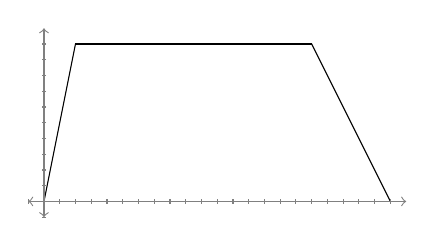
\begin{tikzpicture}[xscale=.2,yscale=.2]
\draw plot[variable=\t,samples=20,domain=0:2] ({\t},{5*\t});
\draw plot[variable=\t,samples=20,domain=2:17] ({\t},{10});
\draw plot[variable=\t,samples=20,domain=17:22] ({\t},{10-2*(\t-17)});
\draw[->,gray] (0,0)--(0,11);
\draw[->,gray] (0,0)--(0,-1);
\draw[->,gray] (0,0)--(-1,0);
\draw[->,gray] (0,0)--(23,0);
\foreach \x in {-1,...,22}
	\draw[gray] (\x,4pt) -- (\x,-4pt);
\foreach \y in {-1,...,10}
	\draw[gray] (4pt,\y) -- (-4pt,\y);
\end{tikzpicture}  
\end{center}

\begin{enumerate}
 \item Set up an initial value problem whose solutions is the position of the rocket after any time $t$. The right hand side should be written in terms of Heaviside functions, where the discontinuities occur after 2, 17, and 22 seconds.
 \item Use Laplace transforms and technology to solve your IVP. Let the computer do all the solving.  The goal is to just GET a solution, and then we'll interpret it.
 \item The rocket will eventually get stuck in the Jello.  How far will it travel before the rocket stops moving? See the side for a hint.\marginpar{Why must every term in the problem that involves an exponential eventually vanish?  What's left over after you ignore all these terms?}
\end{enumerate}

\end{problem*}

}













%\subsection{The Dirac-Delta distribution $\delta(t-a)$ and impulses. }


\newcommand{\DiracIntroComparingHammerAndMagnet}{
What happens if we hit a mass-spring system with a hammer? A hammer blow applies a really large force over a very small amount of time.  To analyze this scenario, we could instead place a magnet underneath a magnet brick that is attached to a spring, and the pull the brick down. We'd have to leave the magnet on for a while to get the brick to come down. With the magnet, we can apply a small force over a long period of time. 
If we hit the brick with a hammer, the blow occurs almost instantly, and yet could result in the exact same downward pull as the magnet.

This problem has you develop the connection between magnets and hammer blows. You should see that a hammer blow is like having an infinitely strong magnet on for no time, which is precisely how we defined the dirac delta.   

\begin{problem}
 Consider a mass-spring system with $m=1$ kg, $c=3$ kg/s, and $k=2$ kg/s$^2$.  Initially the system is at rest (so $y(0)=0$ and $y'(0)=0$). At $t=1$, we turn on a magnet underneath the brick. Let's vary the strength of the magnet, and the length of time we leave the magnet on, and then solve the IVP $y''+3y'+2y=r(t)$, $y(0)=0$, $y'(0)=0$. 
\begin{enumerate}
 \item
 Solve the IVP if the magnet pulls down with a force of 10 N for 1 second so that $r(t)=-10[u(t-1)-u(t-2)]$. This is the only one you should solve by hand.
 \item 
If we doubled the force of the magnet and left the magnet on for half the time, we'd need use $r(t)=-20[u(t-1)-u(t-(1+1/2))]$. 
If we quadrupled the force, and quartered the time the magnet was on, we'd need $r(t)=-40[u(t-1)-u(t-(1+1/4))]$.
If we times the force by 20, but leave the magnet on for one twentieth the time, what should $r(t)$ equal?  
\item 
If we leave the magnet on for $h$ seconds, what should $r(t)$ equal?  
\item 
Our goal is to understand what happens to a mass spring system if we continue to decrease the time the magnet is on, but correspondingly increase the force.   To do this, we need to solve the ODE
$$y''+3y'+2y=-\frac{10}{h}[u(t-h)-u(t-(1+h))].$$
Rather than solve this ODE by hand, let's use technology to visualize the solution.  
Open the Sage worksheet \href{http://bmw.byuimath.com/dokuwiki/doku.php?id=hammer\_blow\_and\_magnet\_comparison}{``Hammer Blow and Magnet Comparision.''} This worksheet shows the position of the spring during the first 10 seconds if we let $h=1,1/2,1/4,1/20$. Try changing it so $h=1/100$ and $h=1/10000$.  Describe what happens to the graph of the solution as $h\to 0$.
\end{enumerate}
\end{problem}
}






%If I introduced the convolution theorem first, then I could define the dirac by looking at the convolution theorem.  That could be a fun way to look at this problem.  


%This needs revamping. I have some goals:  (1) draw stacking tower of functions to describe the dirac.  (2) Show that the derivative of the dirac, (3) Show the sifting theorem.....  Can I do all three of these with one fell swoop?  that would be cool.
% \begin{problem}
% Consider the function 
% $$f_h(t) = 
% \begin{cases}
%  \frac{1}{h} & 0\leq t<h\\
% 0 & \text{otherwise}
% \end{cases} = \frac{1}{h}(u(t-0)-u(t-h)).$$ This function represents a pulse of strength $1/h$ for $h$ seconds.  We would like to examine what happens to this function as $h\to 0$ (so that we have a really strong pulse held for almost no time).
% \begin{enumerate}
%  \item For $h=1$, draw the function $f_1(t)$ for $0\leq t\leq 2$ and compute $\int_0^\infty f_1(t)dt$. Did you get a function that went from 0 to some constant height, and then back to zero?
%  \item Repeat the previous part if $h=1/2$, $h=1/4$, and $h=1/10$.
%  \item If $u(t)$ is the Heaviside function, then compute both $\dfrac{u(h)-0}{h}$ and $u(h)$ at $h=1,1/2,1/4,1/10$.
%  \item What patterns do you see?  If someone asked you to compute $\lim_{h\to 0}f_h(t)$ and $\lim_{h\to 0}\int_0^\infty f_h(t)dt$, what would you give as answers?
% \end{enumerate}
% \end{problem}

% \begin{problem}[$\mathscr{L}\{\delta(t-a)\} = e^{-as}$]
% Complete the following:
% \begin{enumerate}
%  \item 
% Prove that the  Laplace transform of the Dirac delta distribution is $\mathscr{L}\{\delta(t-a)\} = e^{-as}$ (look at the definition above).
%  \item
% Then consider the IVP $y^\prime = \delta(t-5),y(0)=0$.  Use $\mathscr{L}\{\delta(t-a)\} = e^{-as}$ to solve this IVP.  
% When you are done, you'll have found a function whose derivative is $\delta(t-5)$.
%  \item 
%  Use your solution to give a function whose derivative is $5\delta(t-3)$.
% \end{enumerate}
% \end{problem}

% From the previous problem, you should have observed that the derivative of the Heaviside function is the Dirac delta distribution. 
% \begin{theorem}
%  If $u(t-a)$ is the Heaviside function, and $\delta(t-a)$ is the Dirac delta distribution, then 
% $$\frac{d}{dt}u(t-a) = \delta(t-a).$$
% The derivative of a Heaviside is a Dirac delta.
% 
% Engineers often refer to both of these as singularity functions, and use the notation $\left<x-a\right>^0$ for the Heaviside, and $\left<x-a\right>^{-1}$ for the Dirac delta. 
% \end{theorem}


\newcommand{\RCCircuitWithBatteryBetweenTwoAndFourSeconds}{
We now have all the tools we need to solve some pretty cool electricity and mass-spring problems.  We couldn't tackle any capacitors in our discontinuous problems before now, because we would have needed to compute the derivative $E'(t)$.  Now that we have derivatives of Heavisides (namely Dirac deltas), we can solve these problems. 

\begin{problem}
\marginpar{Remember that the key ODE is $LI'+RI+\frac{1}{C}Q=E$.  We have to compute $E'$ as there is a capacitor in the problem.}% 
Consider an $RC$ circuit with $R=2$ and $C=1/8$.  
Suppose that the capacitor has no charge on it, and there is no current flowing at $t=0$.  At $t=2$, we connect a 12 V battery to the circuit.  Then at $t=7$ we remove the battery.  Set up an IVP that would give the current at any time $t$, and then solve the IVP.  Use software to construct a graph of your solution. [Hint: There are no partial fraction decompositions in this one, so it should be REALLY fast.] 
\end{problem}
}

\newcommand{\HamerHitsSpring}{
\begin{problem}
Consider a mass spring system with no friction.  Let $m=1$ and $k=9$. We'll examine what happens if a hammer hits the system.
Suppose the spring is initially at rest at equilibrium.  After 3 seconds, a hammer hits the spring downwards with a force of $10$ N (so $r(t) = -10\delta (t-3)$). The mass-spring system starts to oscillate. Set up and solve an IVP what would give the position of the spring at any time $t$, and state the amplitude of the oscillation. [Again, there are no partial fraction decompositions on this problem, so it should go quite fast.]
\end{problem}
}


\newcommand{\RLCCiruitWithRampTurnedOfAtSixSeconds}{
\begin{problem}
\marginpar{Remember that the key ODE is $LI'+RI+\frac{1}{C}Q=E$.  We have to compute $E'$ as there is a capacitor in the problem.} 
Consider an $RLC$ circuit, with $R=6$, $L=1$, and $C=1/10$. Suppose that at $t=0$ there is no charge on the capacitor, and no current in the wire. We attach a variable voltage source to the RLC circuit, $E(t) = 2t$, and ramp up the power for the first 6 seconds.  After 6 seconds, the voltage drops to zero.  This gives us $E(t) = 2t(1-u(t-6))$.  Set up and solve an IVP that would give the current in the wire after $t$ seconds. 
\end{problem}
}



\newcommand{\StrengthofMaterialsConnectionOptionalProblems}{
\begin{problem*}
\marginpar{If you have had strength of materials, then this problem connects how you use use Heaviside and Dirac delta to tackle all the problems in strengths. You can also use this to solve problems in Statics. You can use it to solve any problem where you have a distributed load (use Heavisides to turn it on and off), and a point force (Dirac delta).} If you have a beam, and you know there is a distributed load on the beam, with a point force applied at another spot on the beam, can you compute the shear stress and the moment at any point in the beam?  This is exactly the same question as finding the  Velocity and position of an object, provided you know the acceleration on the rocket (some external driving force turned on/off based on time) and the rocket is hit by hammers, or meteors (dirac delta) at various points along its path.

I'll be talking about this problem on the next optional day (the day I cancel class while you are getting ready for the exam).
\end{problem*}
}

%I'd really like to do this in the future.  Maybe a cub scout space derby, ask how far the rocket travels.  Maybe a rocket in space, ask what speed it reaches.  Do a rocket from the ground, and ask how high it reaches.  I would like to see ALL of these.  Incorporate them into #15.  Currently 15 is great because mathematica has some really bad Oscillations because of round off error.
%\begin{problem}
%Have them set up 2-3 IVPS. Just state the IVP. We'll solve them in class and look at the solutions.  Maybe they should guess what the graph looks like, and then we'll check in class if they are correct. (or they can use software to solve).
%\end{problem}

\newcommand{\ConvolutionIntroduction}{
We've already seen that the Laplace transform of the product $f\cdot g$ of two functions is not the product of the Laplace transform of each ($L(fg)\neq L(f)L(g)$). Is there some kind of product rule for transforms?  This question led mathematicians to invent what we now call a convolution.  They discovered that the Laplace inverse of $H(s) = L(f)L(g)$ is equal to the quantity $h(t) = (f * g) (t) = \int_0^t f(p)g(t-p)dp$. We call this the convolution of $f$ and $g$. \marginpar{Problem \ref{proof of convolution theorem} has you prove this theorem, which requires that you review double integration and swapping the order of integration.} The variable $p$ is a dummy variable of integration, and we could call it anything else. Some books use $\tau$, but I find it really hard to distinguish between $t$ and $\tau$ when I'm writing on paper, so I use $p$ instead. 
\begin{definition}[Convolutions]
 If $f(t)$ and $g(t)$ are function, then we define the convolution of $f$ and $g$ to be 
$$ (f * g) (t) = \int_0^t f(p)g(t-p)dp.$$
\end{definition}
\begin{theorem}[The Convolution Theorem]\label{the convolution theorem}
 If $f(t)$ and $g(t)$ have Laplace transforms $F(s)$ and $G(s)$, then the inverse Laplace transform of $F(s)G(s)$ is the convolution
$$\mathscr{L}^{-1}\{F(s)G(s)\} = (f * g)(t).$$
This is as close as we get to an inverse product rule for Laplace transforms. 
\end{theorem}

We need to practice the convolution theorem.  It's just an integral.
\begin{problem}
Do the following:
\begin{enumerate}
 \item Show that $1*1 = t$. You'll need to compute $\ds \int_0^t f(p)g(t-p)dp = \int_0^t 1\cdot 1 dp$. 
 \item Compute $1*t$ and $t*1$. You'll need to compute $\ds \int_0^t f(p)g(t-p)dp = \int_0^t 1\cdot (t-p) dp$ and $\ds \int_0^t f(p)g(t-p)dp = \int_0^t p\cdot 1 dp$. 
 \item Compute $t*t$. Compare this to the inverse transform of $\frac{1}{s^2}\frac{1}{s^2}$.
 \item Compute $\sin(t)*t = \int_0^t \sin(p)(t-p)dp$.  You'll want to use integration by parts. 
\end{enumerate}
\end{problem}
}

\newcommand{\PracticeConvolutionWithExponentialAndDiscoverCommutativeRule}{
\begin{problem}
Compute $t*e^{-3t}$ and $e^{-3t}*t$. Which is easier? What is the Laplace inverse of $\dfrac{1}{s^2}\dfrac{1}{s+3}$?
\end{problem}
}

\newcommand{\UseConvolutionToSolveTwoODEs}{
\begin{problem}
Complete each of the following:
\begin{enumerate}
 \item  Compute the convolution $\sin(2t)*1$. Then solve the IVP $y''+4y = 1$, $y(0)=0$, $y'(0)=0$. 
 \item  Compute the convolution $\sin(3t)*t$. Then solve the IVP $y''+9y = t$, $y(0)=0$, $y'(0)=0$. 
\end{enumerate}
\end{problem}
}

\newcommand{\ConvolutionsAndModificationRuleWithSine}{
\begin{problem}
 We've been using the modification rule when we have double complex roots. Use convolutions to find the Laplace inverse of $$\dfrac{1}{(s^2+9)^2}=\dfrac{1}{s^2+9}\dfrac{1}{s^2+9}.$$
\end{problem}
}


\newcommand{\CompareThreeWaysOfSolvingAnODE}{
\begin{problem}
 Consider the IVP $y''+5y'+6y=0$, $y(0)=0$, and $y'(0)=1$. Solve this IVP in three ways.
\begin{enumerate}
 \item Laplace both sides, and then use a convolution (no partial fraction decomposition) to obtain a solution.
 \item Laplace both sides, but use a partial fraction decomposition.
 \item Obtain the homogeneous solution using the characteristic equation, and then use the initial conditions to obtain the constants.
\end{enumerate}
  We'll compare your three solutions in class, and discuss why someone would care about the convolution approach (if you don't see why it's so cool as you use it).
\end{problem}
}



\newcommand{\ProofOfConvolutionTheorem}{
If you'd like to know why the convolution theorem works, please complete the next problem. It requires that you can swap the order of integration on a double integral. Otherwise, feel free to move on to the next problem. If you want a fun puzzle, do this one. 
\begin{problem*}\label{proof of convolution theorem}
 Prove the convolution theorem (Theorem \ref{the convolution theorem}).  Here are some hints.
\begin{itemize}
 \item Let $F(s) = \int_0^\infty f(t) e^{-st}dt$ and then use $G(s) = \int_0^\infty g(w)e^{-sw}dw$. (Why can I use $w$ instead of $t$?)
 \item Explain why $$F(s)G(s) = \int_0^\infty\int_0^\infty f(t) g(w) e^{-s(t+w)}\, dw\, dt.$$
 \item Do a $p$ substitution $p=t+w$ on the inside integral.  You should have something like 
$$F(s)G(s) = \int_0^\infty\int_t^\infty ?e^{-s(p)}\, dp\, dt.$$
 \item Swap the order of integration so that $t$ is inside and $p$ is outside.  This will require that you draw the region of integration in the $tp$ plane.
 \item Show that 
$$F(s)G(s) = \int_0^\infty\left[\int_0^p f(t) g(t-p) \, dt \right]e^{-sp}\, dp.$$ Why does this complete the theorem?
\end{itemize}
\end{problem*}
}





\newcommand{\ConvolutionWithOneGivesIntegralMinusInitialCondition}{
\begin{problem}\label{convolution theorem applied to derivatives and 1}
 Let $f(t)$ be a differentiable function.  
\begin{enumerate}
 \item Show that $f'(t)*1 = f(t)-f(0)$.  
 \item Use the previous part to quickly compute the convolutions $1*1$, $t*1$, $t^2*1$, $\cos(t)*1$, $\sin(\omega t)*1$, and $e^{at}*1$.
 \item The convolution theorem $\mathscr{L}^{-1}\{F(s)G(s)\}=f(t)*g(t)$ allows us to quickly rephrase each of the preceding computations.  For example, we can write the rule $1*t=t^2/2$ using the convolution theorem as $\mathscr{L}^{-1}\left\{\frac{1}{s}\frac{1}{s^2}\right\}=t^2/2$. Rewrite the rule $\sin(\omega t)*1 = \frac{1}{\omega}-\frac{1}{\omega}\cos(\omega t)$ in this way.   
\end{enumerate}
\end{problem}
}

\newcommand{\ObtainTheDiracAsTheDerivativeOfTheHeavisideWithConvolutions}{
\begin{problem}[Discovering the Dirac Delta $\delta(t-a) = u'(t-a)$]\label{obtaining the dirac as the derivative of the heaviside}
 In problem \ref{convolution theorem applied to derivatives and 1}, we showed that $f'(t)*1 = f(t)-f(0)$ provided $f$ is a differentiable function.  Let's ignore this assumption, and just assume the result $f'(t)*1 = f(t)-f(0)$ holds always. Ignoring assumptions and using results blindly can be dangerous and lead to bogus results. However, it's also a way to make conjectures and find new results that actually do work. When mathematicians find useful results in this fashion (by blinding using tools that have no theoretical backing), they'll search for alternate proofs that the useful results work. This can sometimes take decades to fully complete, during which time other branches of science will often just start using the useful results without having a firm theoretical foundation.  Ask me in class about examples of this if you would like more information.
\begin{enumerate}
 \item Let $f(t)=u(t-a)$, the Heaviside function, where $a>0$.  Explain why $u'(t-a)*1=u(t-a)$. We'll use the notation $\delta(t)=u'(t-a)$.  
 \item Using the convolution theorem $\mathscr{L}^{-1}\{F(s)G(s)\}=f(t)*g(t)$, compute the transform of both sides of $u'(t-a)*1=u(t-a)$.  You know the transform of both $1$ and $u(t-a)$. Use this to show that $\mathscr{L}\{u'(t-a)\}=e^{-as}$.
 \item Construct a graph of $u(t-3)$.  From your graph, explain why the derivative of $u(t-3)$ at $t=2$ is zero. What's the derivative at $t=5$?  What's the derivative at any point other than $t=3$?
 \item If you were forced to state a value for the derivative of $u(t-3)$ at $t=3$ and saying, ``it's not differentiable at $t=3$,'' is not an allowed answer, what answer would you give? It's OK to be wrong here. Just make sure you give an answer, and then write a sentence or two to explain why you gave this answer. 
\end{enumerate}
\end{problem}

Because of our work above, let's make a definition
\begin{definition}[Dirac Delta Distribution (or function)]
We define the Dirac delta distribution to be the ``function'' 
$$\delta(t-a) = \begin{cases}0 &t\neq a\\\infty &t=a\end{cases}.$$ 
\begin{itemize}
 \item The Dirac delta $\delta(t-a)$ is not really a function, because the output is $\infty$ (not a real number) at a single point.
\item The derivative of a Heaviside $u(t-a)$ is the Dirac delta $\delta(t-a)$, which we'll write as
 $$\frac{d}{dt}u(t-a) = \delta(t-a).$$
\item We'll require that the Dirac Delta distribution satisfy the integral sifting property
$$%\int_0^\infty \delta(t-a)dt = 1 \quad \quad \text{and}\quad\quad 
\int_0^\infty g(t)\delta(t-a)dt = g(a).$$
This just means when you multiply a function by the Dirac delta and integrate, you eliminate everything except the function at that single point. The Dirac delta provides a pulse at a single point.
\end{itemize}
Engineers often refer to both $u$ and $\delta$ as singularity functions. They use the notation $\left<x-a\right>^0$ for the Heaviside, and $\left<x-a\right>^{-1}$ for the Dirac delta. In future engineering courses, you'll eventually use $u''(t-a) = \left<x-a\right>^{-2}$ and $u'''=\left<x-a\right>^{-3}$. The last part shows up when analyzing the displacement of a beam when two beams are connected with a pin.
\end{definition}
}


%Review Laplace
%Discontinuous Functions
%Dirac Dist.



\newcommand{\ideaconv}{Convolutions provide an inverse product rule}
\newcommand{\ideaheav}{The Heaviside models discontinuities}
\newcommand{\ideadirac}{The Dirac Delta models impulses}
\newcommand{\idealtp}{Laplace Transform Practice}
\mysubsection{\idealtp}
\ReviewSShiftTheorem
\CompareDistinctRootsToCoshAndSinh
\RLCircuitWithBatteryInsertedAndRemovedUsingMovingInitialConditions
\mysubsection{\ideaheav}
\IntroductionToGraphingPiecewiseDefineFunctions
\DefinitionOfHeavisideAndGraphOfAFewFunctions
\GettingFromAGraphToAHeavisideFunction
\mysubsection{\ideaconv}
\ConvolutionIntroduction
\ProofOfConvolutionTheorem
\PracticeConvolutionWithExponentialAndDiscoverCommutativeRule
%\mysubsection{\idealtp}
%\RLCircuitWithBatteryInsertedAndRemovedUsingShifting %Requires MovingInitialConditions
\mysubsection{\ideaheav}
\DevelopLaplaceTransformOfHeavisideFunction
\PracticeForwardLaplaceOfHeaviside
\PracticeInverseLaplaceOfHeaviside
\mysubsection{\idealtp}
\FirstSimpleRLCircuitIVP
\MassSpringSystemPulledDownByAMagnet
\mysubsection{\ideaconv}
\ConvolutionWithOneGivesIntegralMinusInitialCondition
\mysubsection{\ideadirac}
\ObtainTheDiracAsTheDerivativeOfTheHeavisideWithConvolutions
\DiracIntroComparingHammerAndMagnet
\mysubsection{\idealtp}
\ExtraCompareDistinctRootsToCoshAndSinh
\mysubsection{\ideaheav}
\RLCircuitWithRampUpForce
\mysubsection{\ideadirac}
\RCCircuitWithBatteryBetweenTwoAndFourSeconds
\HamerHitsSpring
\mysubsection{\ideaconv}
\UseConvolutionToSolveTwoODEs
\ConvolutionsAndModificationRuleWithSine
\mysubsection{\idealtp}
\RLCCiruitWithRampTurnedOfAtSixSeconds
\RocketInSpaceThroughJello
\CompareThreeWaysOfSolvingAnODE




\StrengthofMaterialsConnectionOptionalProblems




\section*{Wrap up}
\addcontentsline{toc}{section}{Wrap Up}

This concludes the chapter.  Look at the objectives at the beginning of the chapter. Can you now do all the things you were promised? 


\begin{problem}[Lesson Plan Creation] \marginpar{This counts as 4 prep problems. My hope is that you spend at least an hour creating your one-page lesson plan.}
Your assignment: organize what you've learned into a small collection of examples that illustrates the key concepts. I'll call this your one-page lesson plan. You may use both sides. The objectives at the beginning of the chapter give you a list of the key concepts. Once you finish your lesson plan, scan it into a PDF document (use any scanner on campus), and then upload the document to I-Learn.
\end{problem}
